\documentclass[a4paper,11pt]{article}

\usepackage[english]{babel}
\usepackage[utf8x]{inputenc}
\usepackage{amsmath}
\usepackage{graphicx}
\usepackage{cite}
\usepackage{hyperref}
\usepackage{fullpage}
% \usepackage{apacite}
\setlength{\parskip}{1.2ex}
\begin{document}

\title{Open Information System: Conceptual schema}
\author{Thomas Perale -- 0546990\\Maximilien Romain -- 0543411\\Felipe Rojas -- 0542569\\Lehal Sherik -- 0543118}
\date{27 October 2017}

\maketitle

\section{Project subject}

Our OWL have seven classes, Category, Ebook, Purchase, Publisher, Author, User, Publisher and Role.

The \emph{User} class represent both an admin or a customer of the platfrom, it have seven attributes:

\begin{itemize}
  \item userId
  \item information
  \item name
  \item email
  \item password
  \item lastName
\end{itemize}

A \emph{User} of the system can either have the \emph{AdminRole} or just have the \emph{ClientRole},
relation like \emph{hasAdminRole} or \emph{hasClientRole} from the \emph{User} domain in the
\emph{AdminRole}/\emph{ClientRole} range.
Both \emph{AdminRole}/\emph{ClientRole} are subclasses of \emph{Role} they are used to be more specific
what permission a \emph{User} have but are characterized by the attributes:

\begin{itemize}
  \item roleId
  \item description
\end{itemize}

Having one of these role imply the \emph{User} can interract with the \emph{Ebook} has shown with
the relations \emph{hasPurchased} and \emph{manage}. \emph{Ebook} are the main component of the platform
because it's simply what we sell on it. They are defined by:

\begin{itemize}
  \item ISBN
  \item title
  \item year
  \item version
\end{itemize}

But also a remote \emhpt{Author} class bound to \emph{Ebook} by the \emph{hasWritten} class who have got the
following attributes:

\begin{itemize}
  \item authorId
  \item firstName
  \item lastName
\end{itemize}

Also defined with the \emph{Publisher} class bound from \emph{Ebook} by the relation \emph{isPublishedBy},
it is made of:

\begin{itemize}
  \item publisherId
  \item name
\end{itemize}

And finally \emph{Categorie} class bound by \emph{Ebook} by the \emph{hasCategory} relation, categories are just
a way to do search on ebooks by genre so the \emph{Category} class is defined by:

\begin{itemize}
  \item categoryId
  \item description
\end{itemize}

To enable customers to read ebooks they must first create \emph{Purchase} as you can see in our ontology a \emph{User}
make by the \emph{isMaking} relation \emph{Purchase}. \emph{Purchase} are a way to modelize ebooks the user paid to have
for each \emph{Purchase} the user have to make a transaction and they can contain more than one \emph{Ebook} has we can
see with the \emph{isPartOf} relation.

Other privilege a customer have is to rate the \emph{Ebook} he bought modelized by the \emph{Rating} class.
\emph{User} and \emph{Rating} are bound together by the \emph{hasRated} relation and make \emph{Ebook} in relation
with it with \emph{hasRating}. The attributes for \emph{Rating} are:

\begin{itemize}
  \item ratingId
  \item number
\end{itemize}

\section{Rules description}


First rule, If the book belongs to a category and that category is also a subcategory to another
category, it implies that the book belongs to both the main category and it's subcategory.\\

Ebook(?x), Category(?y), Category(?z), subCategoryOf(?y, ?z), hasCategory(?x, ?y), differentFrom(?y, ?z) $\rightarrow$ hasCategory(?x, ?z)

Is relevant because an ebook could have more than one cateogory and one of those categories could
be a subcategory of one of these, which means that the ebook will have a category and a subcategory.
Example- If a book belongs to "war" category and the "war" category belongs to "action" category,
it is implied that the book belongs to both "war" and "action" categories.

Second rule, If a user makes a purchase and an ebook is part of the purchase, then we can imply that
the user “HasPurchased” an ebook. \\

User(?x), Purchase(?y), Ebook(?z), isMaking(?x, ?y), isPartOf(?z, ?y) $\rightarrow$ hasPurchased(?x, ?z)

This rule is relevant because a purchase needs at least one eBook to be purchased by an user, meaning
that a user purchased an eBook.

Third rule, If a user is rating an eBook or an eBook has been rated implies that the user hasPurchased an ebook.
The rule is relevant because users who didn't purchase the book can't rate it.\\

User(?x), Rating(?y), Ebook(?z), hasRated(?x, ?y), hasRating(?z, ?y) $\rightarrow$ hasPurchased(?x, ?z)

This rule is relevant since only users that has purchased an eBook would be able to rate that eBook.

The last rule implies that if a user has the role "admin", they can manage the ebooks database on the system.\\

User(?admin), Ebook(?book), AdminRole(?role), hasAdminRole(?admin, ?role) $\rightarrow$ manage(?admin, ?book)

This rule is relevant because an Admin should be the only type of user that can manage the eBooks.

\section{ER Schema}

\begin{center}
  \makebox[\textwidth]{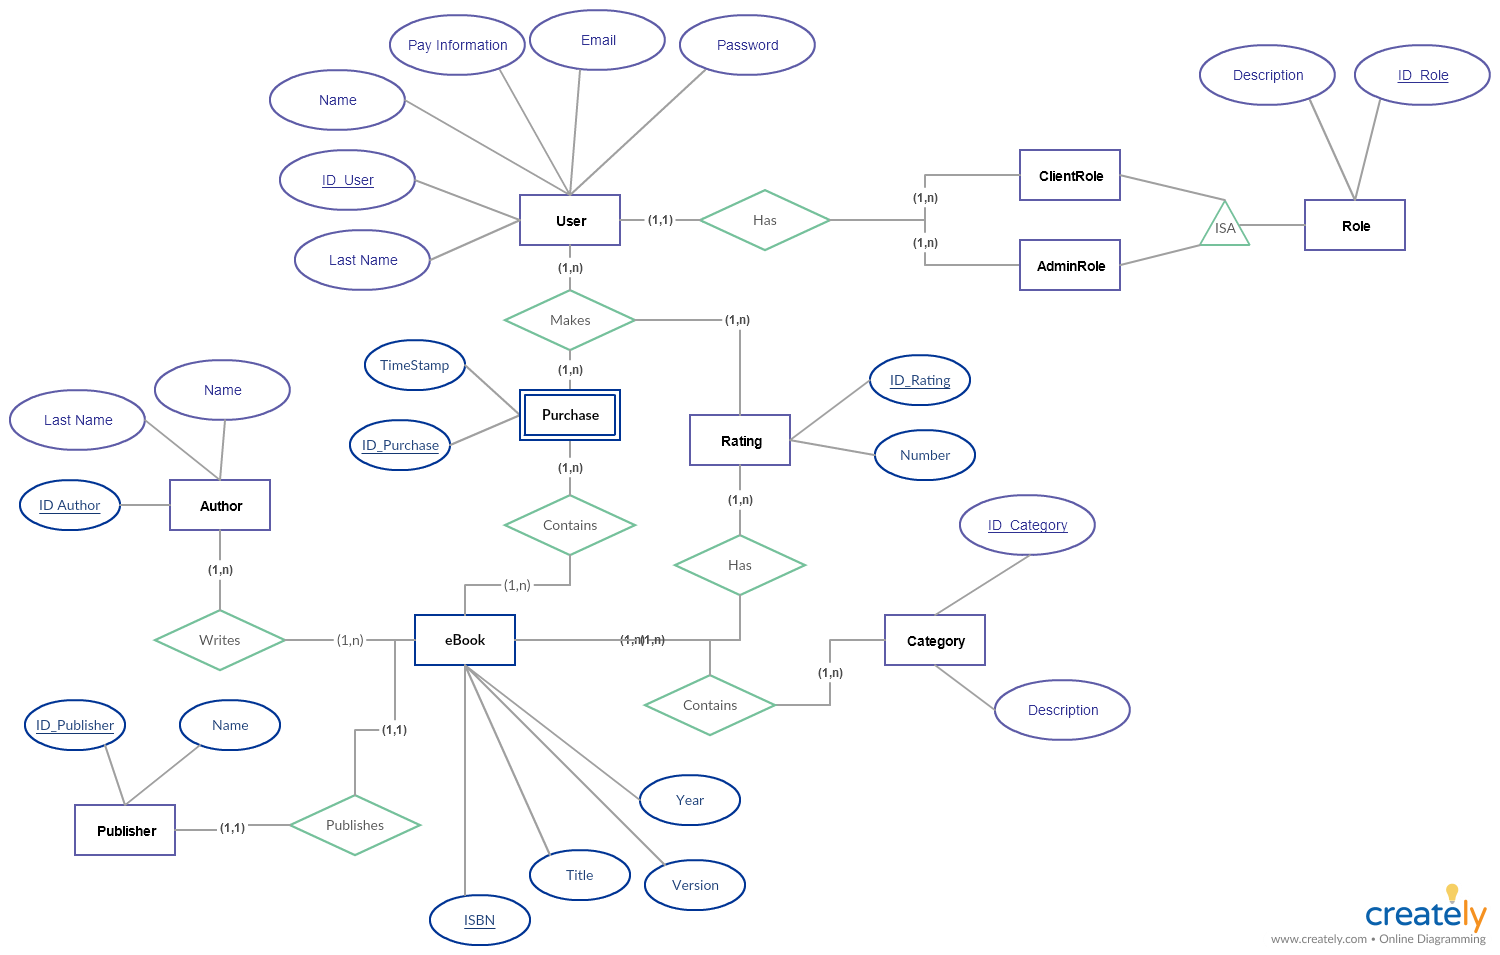
\includegraphics[width=\paperwidth]{ER_graph.png}}
\end{center}

\section{WebOwl visualisation}
\begin{center}
  \makebox[\textwidth]{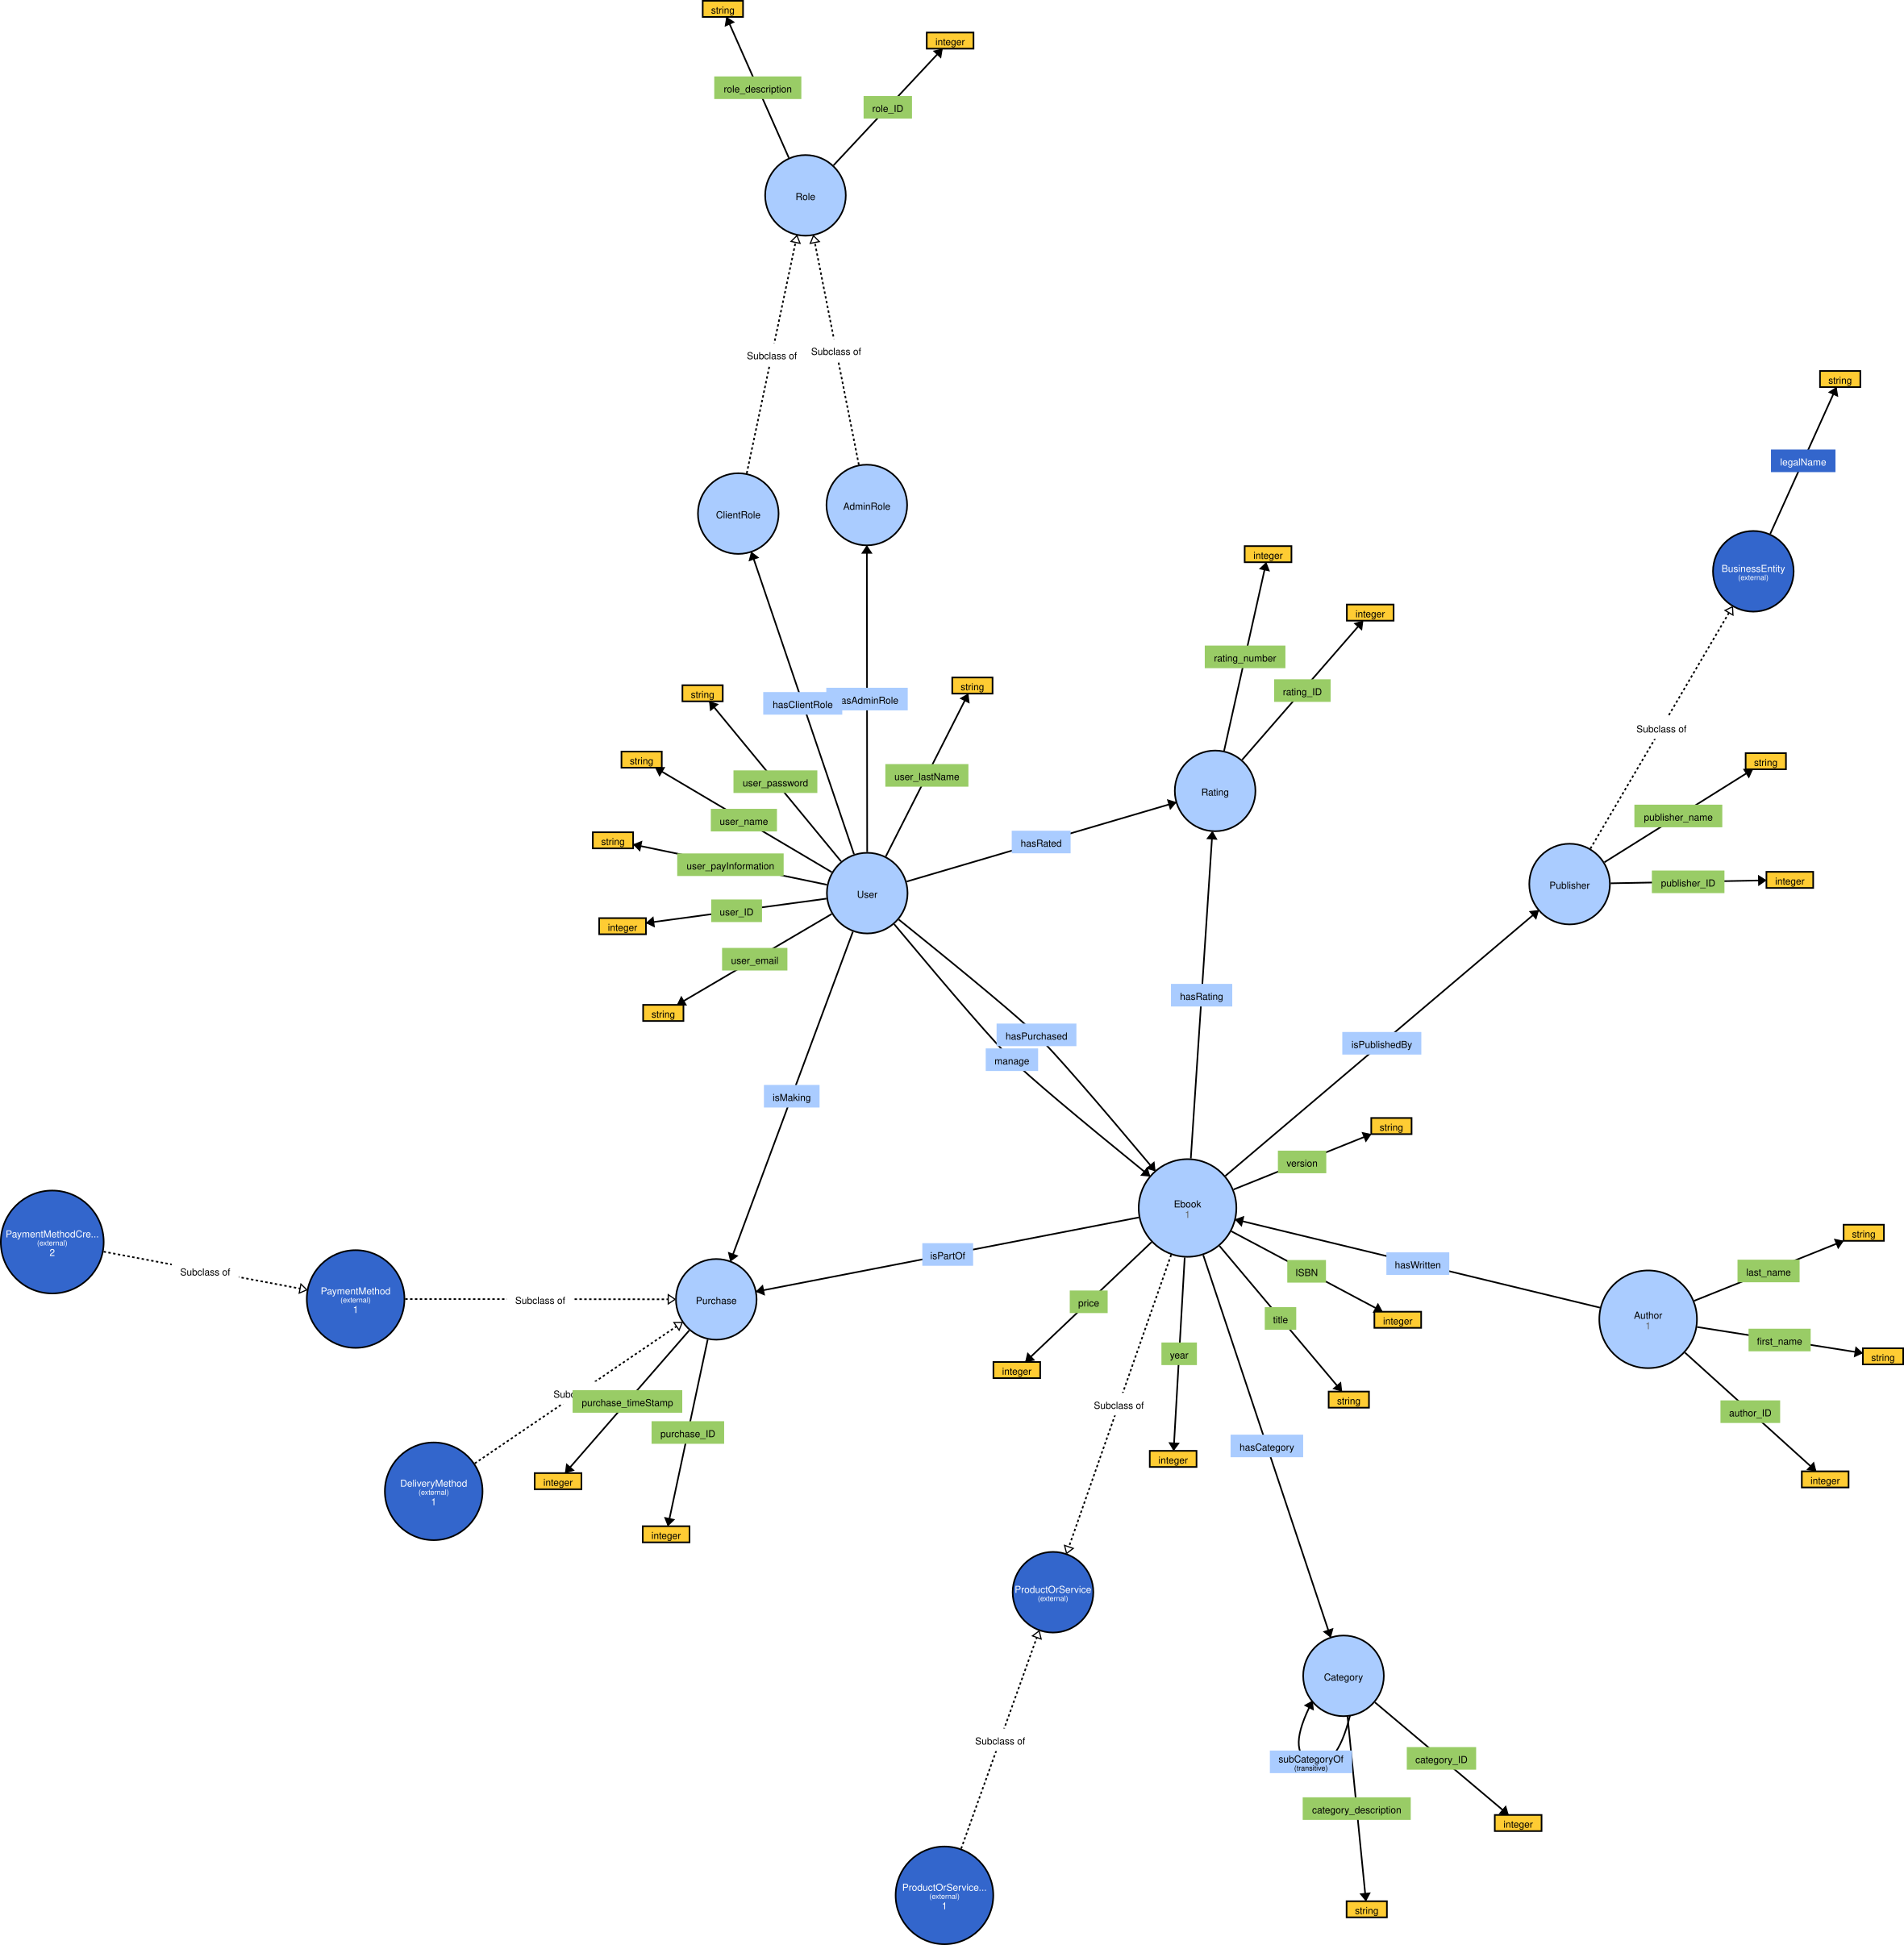
\includegraphics[width=\paperwidth]{webOwl.png}}
\end{center}


\end{document}
